%===========================================================================


\section{Variance Decomposition and Hypothesis Verdicts \texorpdfstring{[C]}{[C]}}
\label{sec:decomposition}
%===========================================================================

This section assembles the preceding estimates into the variance decomposition
and the six hypothesis verdicts. The label spread is read across the three
variants of Section~\ref{sec:internal_performance}, the model-class spread
across the model rows of the same table, the split contrast against the
random-split arm, and the transport contrast against the external estimates of
Section~\ref{sec:external_validation}. Each is an AUROC contrast with an interval
from the same stay-level cluster bootstrap.

\paragraph{Spreads as ranges.} Each spread is a \emph{range}: the largest AUROC
in a set minus the smallest. The label spread is a range over three variants and
the model-class spread over six specifications. Because a range grows with the
number of values even when the underlying quantities are identical, a range
over six is expected to exceed one over three by roughly half again, a bias
present in every bootstrap replicate (the same reason the subgroup range is not
treated as an effect size in Section~\ref{sec:equity}).

The ordering does not depend on this statistic. The model-class range spans a
structural gap rather than sampling scatter, between the two fitted
models and the four rule-based and Cox comparators, and \emph{any} single
contrast across that gap is larger than the whole label range. The narrowest of
them, GBT against the Cox model, is \pcAurocGbtB{} against \pcAurocCoxB, which
exceeds the label range by a factor of eight and involves no order statistic.
An asymmetry of about half again cannot account for \pcSpreadModelClass{}
against \pcSpreadLabel.

A variance-components partition is not used, for two reasons: the AUROCs are
computed on the same test rows, so the design supplies no suitable error term,
and \S7 of the pre-registration fixed the estimand as the \emph{spread}. The
range is reported as a descriptive summary with a bootstrap interval.

Two of the six hypotheses admit no test statistic, for reasons of design; both
still occupy a slot in the correction (Section~\ref{sec:confirmatory_verdicts}).

\subsection{The Decomposition Table}

\begin{table}[H]
    \centering\small
    \begin{tabular}{p{4.6cm}cll}
        \toprule
        \textbf{Factor (others fixed)}         & \textbf{$\Delta$AUROC} & \textbf{95\% CI} & \textbf{H} \\
        \midrule
        Model class (label B, temporal)        & \pcSpreadModelClass & \pcSpreadModelClassCiLo--\pcSpreadModelClassCiHi & n/a \\
        Label definition (primary, temporal)   & \pcSpreadLabel      & \pcSpreadLabelCiLo--\pcSpreadLabelCiHi & H1 \\
        Split method (primary, label B)        & \pcSpreadSplit      & \pcHFourCiLo--\pcHFourCiHi & H4 \\
        External transport (primary, label B)  & \pcSpreadMetric     & \pcHFiveCiLo--\pcHFiveCiHi & H5 \\
        \midrule
        GBT $-$ primary (label B, temporal)    & \pcHSixEst          & \pcHSixCiLo--\pcHSixCiHi & H6 \\
        \bottomrule
    \end{tabular}
    \caption{Variance decomposition with 95\% stay-level cluster-bootstrap
    intervals. The name is the pre-registration's (\S1) and the quantities are
    ranges, not variance components: they neither estimate nor partition a
    variance, and they are not on a common denominator, so they cannot be
    summed or expressed as shares of a total. Each row varies one factor with
    the others held fixed, over the alternatives named. The first row tests no
    hypothesis; H1 contrasts it with the label range. H6, below the rule, is the
    contrast between the two \emph{flexible} estimators alone.
    \textbf{[C] confirmatory.}}
    \label{tab:decomposition}
\end{table}

The four factors differ widely in effect. \textbf{The spread across the six
evaluated model specifications is the largest} (\pcSpreadModelClass). That set
runs from a 29-term dynamic hazard model to qSOFA and differs in features,
event handling and fitting as well as model form (Section~\ref{sec:models}), so
the claim concerns this comparison, not model architecture in general.
\textbf{External transport has the second-largest point estimate}
(\pcSpreadMetric), but its interval is the widest in the table and covers zero,
so its rank is not established. The label moves discrimination by
\pcSpreadLabel{} and the split by \pcSpreadSplit, both small, and the split's
interval covers zero. The pre-registered expectation that the four factors
would be comparable is not supported. Three qualifications apply:

\begin{itemize}
    \item Between the two \emph{flexible} estimators, fitted on identical
          covariates, the gap is \pcHSixAbsEst{}, an order of magnitude below
          the six-specification range and of the same order as the label's
          (H6; Section~\ref{sec:h6}).
    \item The label factor is small \emph{in discrimination} only. The
          variants disagree about which patients are septic
          ($\kappa = \pcKappaVsBA$, A vs B), so they define different cohorts,
          prevalences and denominators for every downstream clinical claim.
    \item The split interval [\pcHFourCiLo, \pcHFourCiHi] excludes the
          pre-registered $+0.02$ optimism threshold while covering zero. The
          transport row rests on \pcExtNEventsB{} events, and its interval
          [\pcHFiveCiLo, \pcHFiveCiHi] contains both zero and a degradation
          twice the size of the label effect.
\end{itemize}

\subsection{Corrected Confirmatory Verdicts}
\label{sec:confirmatory_verdicts}

\begin{table}[H]
    \centering\footnotesize
    \adjustbox{max width=\textwidth}{%
    \begin{tabular}{llrlr>{\raggedright\arraybackslash}p{3.6cm}}
        \toprule
        \textbf{H} & \textbf{Contrast $\theta$} & \textbf{Est.} & \textbf{95\% CI}
        & \textbf{$p_{\text{Holm}}$} & \textbf{Verdict} \\
        \midrule
        H1 & Label spread $-$ model spread   & \pcHOneEst   & \pcHOneCiLo--\pcHOneCiHi   & \pcHOnePHolm   & \pcHOneVerdict   \\
        H2 & Unstable covariates (count)     & \pcHTwoEst   & n/a                         & n/a             & Descriptive      \\
        H3 & Pre-treatment onsets (count)    & \pcPreTreatOnsetsVarB & n/a               & n/a             & Definitional     \\
        H4 & Random $-$ temporal AUROC       & \pcHFourEst  & \pcHFourCiLo--\pcHFourCiHi & \pcHFourPHolm  & \pcHFourVerdict  \\
        H5$^{\dagger}$ & Internal $-$ external AUROC$^{\dagger}$ & \pcHFiveEst  & \pcHFiveCiLo--\pcHFiveCiHi & \pcHFivePHolm  & \pcHFiveVerdict  \\
        H6 & GBT $-$ primary AUROC           & \pcHSixEst   & \pcHSixCiLo--\pcHSixCiHi   & \pcHSixPHolm   & \pcHSixVerdict   \\
        \bottomrule
    \end{tabular}}
    \caption{The confirmatory family. One-sided cluster-bootstrap tests against
    each hypothesis's pre-registered threshold ($\theta_0 = 0$ for H1, and for
    the amended AUROC transport contrast shown in H5's reserved slot; 0.02 for
    H4 and H6), Holm--Bonferroni corrected at family size $m = 6$ and
    FWER 0.05. H2 and H3 reserve a slot without contributing a p-value, which
    makes the correction on the other four stricter. H3's count is entailed by
    the onset rule (Proposition~\ref{prop:h3}). \textbf{The Verdict column
    reports the pre-registered test only}: H6's non-rejection is not evidence of
    equivalence, and its one-sided non-inferiority is read off the interval
    (Section~\ref{sec:h6}). The smallest reportable p-value is $1/(B+1)$.
    \textbf{[C] confirmatory, except $\dagger$}: H5's pre-registered estimand
    is \textbf{not evaluable}, and the row shows an \textbf{[A] amended,
    post-hoc} substitute contrast occupying its correction slot
    (Section~\ref{sec:h5}).}
    \label{tab:confirmatory}
\end{table}

H1 and H4 are not confirmed: their adjusted p-values are \pcHOnePHolm{} and
\pcHFourPHolm, and their point estimates lie on the opposite side of zero from
the one predicted. H6 is not rejected and its interval supports one-sided
non-inferiority but not two-sided equivalence. H2 is descriptive, and H3 and
H5 were not evaluable as pre-registered; the contrast substituted for H5 is
inconclusive. The following subsections give each verdict with its estimate;
the underlying results are in the sections cited.

\subsection{H1: Label Dominance (Not Confirmed)}

\begin{mdframed}[backgroundcolor=ATUOrange!20, linecolor=ATUOrange]
    \textbf{H1 [C]:} Spread in AUROC across label variants $\geq$ spread across
    model classes.

    \textbf{Point estimates:} label spread $= \pcSpreadLabel$;
    model spread $= \pcSpreadModelClass$.

    \textbf{Contrast:} $\theta = \pcHOneEst$ (95\% CI
    \pcHOneCiLo--\pcHOneCiHi), Holm-adjusted $p = \pcHOnePHolm$.
    \textbf{H1 NOT CONFIRMED; the estimate lies in the direction opposite
    to the one hypothesised.}
\end{mdframed}

Across the six evaluated specifications, model choice affected AUROC more than
the three Sepsis-3 variants did: the difference of spreads excludes zero. The
specification spread runs from rule-based scores (qSOFA \pcAurocQsofaB, SIRS
\pcAurocSirsB, NEWS2 \pcAurocNewsB) through the Cox comparator
(\pcAurocCoxB) to the two flexible estimators (primary \pcAurocPrimaryB, GBT
\pcAurocGbtB). The variants nevertheless changed cohort membership
substantially: A and B agree on only \pcPctAgreeBA\% of stays
($\kappa = \pcKappaVsBA$) despite near-identical prevalence
(Section~\ref{sec:label_anchor_results}).

\begin{figure}[H]
    \centering
    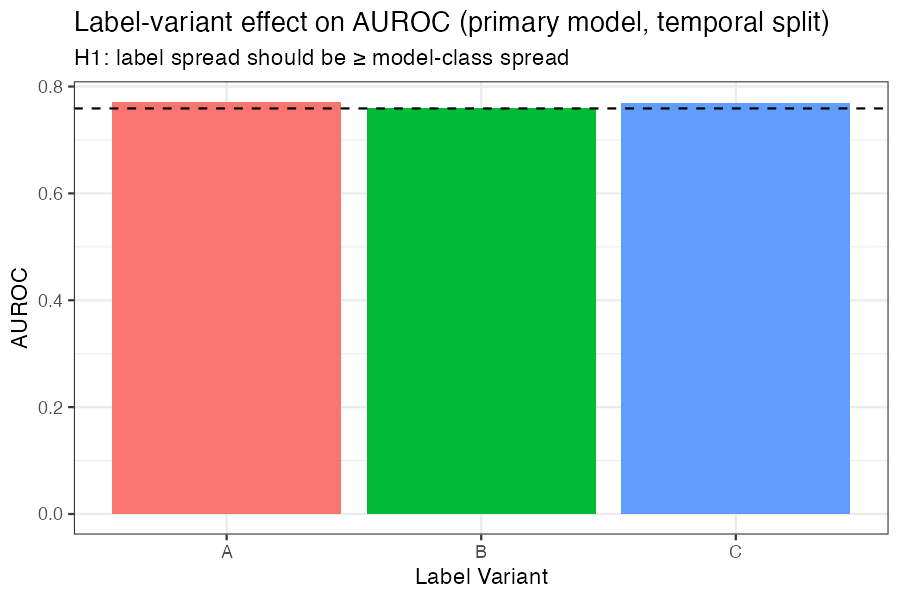
\includegraphics[width=0.85\textwidth]{images/09_label_variance_auroc.png}
    \caption{AUROC by label variant for each model (temporal split). Both
    quantities are \emph{ranges}, largest minus smallest: the range within each
    model group is the label contribution (\pcSpreadLabel, over three variants)
    and the range across groups is the spread across the six model
    specifications (\pcSpreadModelClass), larger by roughly an order of
    magnitude (Section~\ref{sec:decomposition}).}
    \label{fig:label_variance_auroc}
\end{figure}

\subsection{H2: Coefficient Instability (Met, Descriptive)}
\label{sec:h2}

\begin{mdframed}[backgroundcolor=ATUSand!30, linecolor=ATUGreen]
    \textbf{H2 [C]:} At least one feature changes sign or magnitude
    $\geq 2\times$ across label variants.

    \textbf{Result:} of the \pcHTwoNTerms{} covariates shared by all three
    variants, \pcHTwoNSign{} reverse sign, \pcHTwoNMag{} change magnitude by
    $\geq 2\times$, and \pcHTwoEst{} do at least one of the two.
    \textbf{H2's criterion is met (descriptive; no test statistic).}

    \textbf{Multiplicity:} H2 reserves a slot in the confirmatory family of six
    but contributes no p-value, which makes the Holm correction on the
    remaining hypotheses stricter rather than weaker.
\end{mdframed}

The count is the pre-registered answer, reported unmodified, and depends on the
penalised fit of Section~\ref{sec:primary_model_spec}. Because a threshold rule
on point estimates cannot separate genuine movement from imprecision, it is an
upper bound on the instability present.

\begin{table}[H]
    \centering
    \begin{tabular}{lp{8cm}}
        \toprule
        \textbf{Feature}           & \textbf{What changed}                   \\
        \midrule
        Bilirubin                  & Sign reversal across variants           \\
        Any vasopressor            & Sign reversal \emph{and} magnitude $\geq 2\times$ \\
        Platelets                  & Magnitude $\geq 2\times$                \\
        Creatinine measured        & Magnitude $\geq 2\times$                \\
        Platelets measured         & Magnitude $\geq 2\times$                \\
        WBC measured               & Magnitude $\geq 2\times$                \\
        \bottomrule
    \end{tabular}
    \caption{Features with sign reversal or magnitude instability across label
    variants. \pcHTwoNSign{} of the \pcHTwoNTerms{} shared covariates reverse
    sign and \pcHTwoEst{} are unstable on either criterion. Full per-covariate
    flags are in \texttt{12\_h2\_coefficient\_stability.csv}.}
    \label{tab:coef_instability}
\end{table}

\subsubsection{Does the instability exceed its own estimation noise? (Protocol
Amendment 7)}
\label{sec:h2_uncertainty}

Using the cluster-robust covariance (Section~\ref{sec:primary_model_spec}),
the difference between each flagged covariate's two extreme estimates is
referred to their pooled standard error (Table~\ref{tab:h2_uncertainty}).

\begin{table}[H]
    \centering\footnotesize\setlength{\tabcolsep}{4pt}
    \adjustbox{max width=\textwidth}{% GENERATED by thesis_constants.R -- do not edit
\begin{tabular}{lrrrrrrl}
\toprule
\textbf{Covariate} & \textbf{$\beta_A$} & \textbf{$\beta_B$} & \textbf{$\beta_C$} & \textbf{Max diff.} & \textbf{Pooled SE} & \textbf{Ratio} & \textbf{Kind} \\
\midrule
\texttt{wbc\_measured} & 0.0969 & 0.5374 & 0.8989 & 0.8020 & 0.0517 & 15.51 & action \\
\texttt{platelets\_measured} & -0.2563 & -0.5614 & -0.8173 & 0.5610 & 0.0529 & 10.60 & action \\
\texttt{creatinine\_measured} & 0.2877 & 0.2303 & 0.0343 & 0.2534 & 0.1024 & 2.48 & action \\
\texttt{platelets} & 0.0002 & 0.0001 & 0.0003 & 0.0002 & 0.0002 & 1.07 & physiol. \\
\texttt{vaso\_anyTRUE} & -0.0374 & 0.0271 & 0.0025 & 0.0645 & 0.0864 & 0.75 & action \\
\texttt{bilirubin\_total} & 0.0014 & -0.0016 & -0.0020 & 0.0034 & 0.0056 & 0.61 & physiol. \\
\bottomrule
\end{tabular}
}
    \caption[H2 instability against estimation noise]{Each covariate flagged by
    H2, with its coefficient under each label variant, the difference between
    the two extremes, the pooled cluster-robust standard error of those two
    estimates, and their ratio. \pcHTwoNRobust{} of the \pcHTwoNFlagged{}
    flagged covariates move by more than roughly twice their pooled standard
    error; the remaining \pcHTwoNNoise{} move by less, the largest such ratio
    being \pcHTwoZMaxNoise; no covariate falls between \pcHTwoZMaxNoise{} and
    \pcHTwoZMinRobust. ``Kind'' marks clinician action or patient physiology
    (Section~\ref{sec:h2_action}). \textbf{A diagnostic, not a test}: the fits
    share stays, and the covariance is that of the penalised estimator
    (Section~\ref{sec:primary_model_spec}).}
    \label{tab:h2_uncertainty}
\end{table}

The pre-registered count stands; the post-hoc diagnostic (Protocol
Amendment 7) is reported beside it, not in its place. The covariates whose
movement exceeds their standard errors are \pcHTwoNRobustAction{} of
\pcHTwoNRobust{} action-derived, with ratios from \pcHTwoZMinRobust{} to
\pcHTwoZMax, and all are indicators of whether a test was ordered. Both sign
reversals, bilirubin and vasopressor exposure, carry the two smallest ratios,
so no claim rests on either individually. This agrees with the by-kind split
(Section~\ref{sec:h2_action}) and the ablation (Section~\ref{sec:ablation}),
but all three are computed from the same three fitted models and are not
independent corroboration.

\subsubsection{The instability is concentrated in the action-derived features}
\label{sec:h2_action}

The covariates fall into two kinds. \textbf{Action-derived} features record
clinician behaviour (vasopressor exposure and the per-test order indicators);
\textbf{physiological} features record the patient (vital signs, laboratory
values and their rolling slopes). Table~\ref{tab:instability_by_kind} splits the
instability by kind.

\begin{table}[H]
    \centering
    \begin{tabular}{lrrr}
        \toprule
        \textbf{Feature kind} & \textbf{Covariates} & \textbf{Unstable}
        & \textbf{\% unstable} \\
        \midrule
        Action-derived & \pcHTwoNAction & \pcHTwoNUnstableAction & \pcHTwoPctUnstableAction \\
        Physiological  & \pcHTwoNPhysio & \pcHTwoNUnstablePhysio & \pcHTwoPctUnstablePhysio \\
        \bottomrule
    \end{tabular}
    \caption{H2 instability by feature kind. Action-derived covariates are a
    minority of the specification but a majority of the unstable terms.
    \textbf{[E] exploratory.}}
    \label{tab:instability_by_kind}
\end{table}

Instability is concentrated in the features that encode clinician behaviour,
which a change of label affects in a way that a heart rate is not. With
\pcHTwoNTerms{} covariates the counts are small and the difference between the
two rates is not tested. The result supports Lauritsen et al.'s
\cite{lauritsen2021framing} framing-instability concern for specific effect
estimates, not instability of the fitted model as a whole.

\subsection{H3: Treatment Leakage, Definitional and Empirical}
\label{sec:h3}

\begin{mdframed}[backgroundcolor=ATUPurple!10, linecolor=ATUPurple]
    \textbf{H3 [C]:} Restricting to pre-treatment hours reduces AUROC by
    $\geq 0.03$.

    \textbf{Definitional result:} \textbf{\pcPreTreatOnsetsVarB{} sepsis onset
    events} in \pcPreTreatPersonHoursVarB{} pre-treatment person-hours. AUROC is
    undefined, so the pre-registered contrast cannot be formed. This zero is
    \emph{proved} below (Proposition~\ref{prop:h3}) to follow from the onset
    rule used by variants A--C; it is a statement about the implementation, not
    a measurement.

    \textbf{Empirical result (Protocol Amendment 4):} relabelling the same
    stays with the standard $\min(t_{\text{susp}}, t_{\text{SOFA}})$ onset
    (Variant F) moves \pcFNMovedEarlier{} of \pcFNOnsets{} onsets earlier
    (\pcFPctMovedEarlier\%, median \pcFMedianShiftH\,h) and places
    \textbf{\pcPreTreatOnsetsVarF{} onsets before treatment}, identified at
    \pcPreTreatAurocPrimaryF{} AUROC (\pcPreTreatAurocGbtF{} GBT).
    \textbf{H3 is not evaluable as pre-registered; the definitional and
    empirical statements replace it.}

    \textbf{Multiplicity:} like H2, H3 reserves a slot in the confirmatory
    family without contributing a p-value. Variant F's contrast against B is
    exploratory (family E3).
\end{mdframed}

\paragraph{Definitional result.}
In the hours before the first antibiotic or culture there are zero onset events
for variants A--C and E. This follows from how the onset timestamp is assigned:

\begin{mdframed}[backgroundcolor=ATUSand!20, linecolor=ATUGreen]
    \begin{proposition}\label{prop:h3}
    Let $t_{\mathrm{anchor}}$ be the earlier of the first qualifying antibiotic
    order and the first culture draw of an admission, and let
    $t_{\mathrm{onset}}$ be the onset assigned by variants A, B, C or E. Then
    $t_{\mathrm{onset}} \geq t_{\mathrm{anchor}}$ for every labelled stay, so the
    window $[\,\cdot\,,\, t_{\mathrm{anchor}})$ contains no onset.
    \end{proposition}

    \emph{Proof.} Under E, $t_{\mathrm{onset}} = t_{\mathrm{susp}}$, and
    $t_{\mathrm{susp}}$ is defined as the \emph{later} element of a qualifying
    antibiotic-culture pair; both elements are at or after
    $t_{\mathrm{anchor}}$, so $t_{\mathrm{susp}} \geq t_{\mathrm{anchor}}$.
    Under A, B and C the SOFA criterion is a \emph{membership} gate: a stay is
    labelled only if the $\geq 2$-point rise occurs somewhere in the evaluation
    window, but the timestamp written is still $t_{\mathrm{susp}}$
    (Section~\ref{sec:alt_labels}). The inequality therefore carries over
    unchanged. $\square$
\end{mdframed}

\noindent The exact one-sided 95\% upper bound on the pre-treatment onset rate
in the inference tables therefore bounds a quantity the definition fixes at
zero.

\paragraph{Empirical result.}
Under the standard $\min(t_{\text{susp}}, t_{\text{SOFA}})$ onset
(Equation~\ref{eq:early_onset}), an onset precedes the anchor whenever the SOFA
rise is detected before the clinician acts, and Proposition~\ref{prop:h3} does
not apply. Variant F, with the same septic stays as Variant B, records
\pcPreTreatOnsetsVarF{} pre-treatment onsets in the temporal test set,
identified at \pcPreTreatAurocPrimaryF{} AUROC
(Section~\ref{sec:pretreatment_label}). The conjunction-timing rule of the
pre-registered variants is therefore what prevents pre-treatment onsets from
being recorded; Section~\ref{sec:discussion_core} interprets this result.

\subsection{H4: Split Optimism (Not Confirmed)}
\label{sec:h4_discussion}

\begin{mdframed}[backgroundcolor=ATUOrange!20, linecolor=ATUOrange]
    \textbf{H4 [C]:} Temporal-split AUROC is at least 0.02 lower than
    random-split AUROC.

    \textbf{Result:} primary model, random AUROC \pcAurocRandomPrimaryB{}
    against temporal \pcAurocPrimaryB. Difference $= \pcHFourEst$ (95\% CI
    \pcHFourCiLo--\pcHFourCiHi): the temporal split is the \emph{higher} of
    the two. Test against the pre-registered threshold $\theta_0 = 0.02$:
    Holm-adjusted $p = \pcHFourPHolm$. \textbf{H4 NOT CONFIRMED.}
\end{mdframed}

\begin{table}[H]
    \centering
    \begin{tabular}{llrr}
        \toprule
        \textbf{Model} & \textbf{Temporal} & \textbf{Random} & \textbf{Random $-$ temporal} \\
        \midrule
        Primary & \pcAurocPrimaryB & \pcAurocRandomPrimaryB & \pcSplitDeltaPrimaryB \\
        GBT     & \pcAurocGbtB     & \pcAurocRandomGbtB     & \pcSplitDeltaGbtB \\
        Cox     & \pcAurocCoxB     & \pcAurocRandomCoxB     & \pcSplitDeltaCoxB \\
        NEWS2   & \pcAurocNewsB    & \pcAurocRandomNewsB    & \pcSplitDeltaNewsB \\
        \bottomrule
    \end{tabular}
    \caption{Temporal vs.\ random split comparison (Variant B, AUROC). Every
    model scores lower on the random split.}
    \label{tab:split_optimism}
\end{table}

The interval includes zero and excludes $+0.02$, and all four models fitted
under both splits score lower on the random split, by \pcSplitDeltaMinAbs{} to
\pcSplitDeltaMaxAbs. The temporal test set is the 2017--2019 cohort whereas the
random test set spans all years, so the contrast also confounds split design
with cohort composition, and the random split cannot be assumed to be the more
permissive design (Section~\ref{sec:limitations}).

\subsection{H5: Metric Divergence (Not Evaluable as Pre-Registered)}
\label{sec:h5}

\begin{mdframed}[backgroundcolor=ATUOrange!20, linecolor=ATUOrange]
    \textbf{H5 [C]:} Utility Score declines proportionally more than AUROC from
    internal to external validation.

    \textbf{Testable arm:} AUROC degradation internal $\to$ external (primary,
    Variant B) $= \pcHFiveEst$ (95\% CI \pcHFiveCiLo--\pcHFiveCiHi); internal
    \pcAurocPrimaryB, eICU-CRD \pcExtAurocPrimaryB{} on \pcExtNEventsB{}
    external events. Holm-adjusted $p = \pcHFivePHolm$.
    \textbf{The point estimate falls, but the interval does not exclude no
    change.}

    \textbf{Non-testable arm:} the internal Utility Score is
    \pcUtilityPrimaryB{} at the default cut-off and \pcUtilityMaxPrimaryB{} at
    its best threshold, so a proportional decline cannot be formed.
    \textbf{H5 AS PRE-REGISTERED IS NOT EVALUABLE; the substituted AUROC
    contrast is not supported.}
\end{mdframed}

H5's proportional contrast requires a non-zero internal Utility Score, and the
internal score under the primary label is \pcUtilityPrimaryB{} at the default
cut-off and \pcUtilityMaxPrimaryB{} at its best threshold, so the contrast
cannot be formed. Its slot is occupied by the AUROC limb alone (\S13.6 of
\texttt{00\_preregistration.md}), to which the Holm-adjusted \pcHFivePHolm{}
applies. That contrast, \pcHFiveEst{}, is in the predicted direction and about
three-quarters of the 0.085 anticipated from Moor et al.\
\cite{moor2023review}, but its interval is consistent with both no loss and a
loss twice as large, because it rests on \pcExtNEventsB{} external events
(Section~\ref{sec:external_coverage}). The Narrow label loses most and the
Liberal least, and the antibiotic-only arm, a different target on
\pcExtAbxNEventsB{} events, shows a degradation of the same sign
(\pcAurocPrimaryB{} to \pcExtAbxAurocPrimaryB); neither observation is a test.

\subsection{H6: Model-Class Null (Not Rejected; One-Sided Non-Inferiority)}
\label{sec:h6}

\begin{mdframed}[backgroundcolor=ATUSand!30, linecolor=ATUGreen]
    \textbf{H6 [C]:} $|\Delta_\text{AUROC}(\text{GBT} - \text{primary})| \leq 0.02$.

    \textbf{Result:} $\Delta = \pcHSixEst$ (GBT \pcAurocGbtB, primary
    \pcAurocPrimaryB), 95\% CI \pcHSixCiLo--\pcHSixCiHi. The \emph{upper} limit
    lies inside the bound $\theta_0 = 0.02$; the lower limit does not.
    \textbf{H6 NOT REJECTED. The interval supports one-sided non-inferiority
    of the primary model (GBT is not better by more than the margin), not
    two-sided equivalence.}
\end{mdframed}

Both models are scored on the same person-hours, so the contrast is paired,
and the primary model is also ahead under the other two labels
(Table~\ref{tab:internal_results}). The pre-registered form (\S7) places
equivalence in the \emph{null}, $H_0\colon |\theta| \leq 0.02$; \textbf{this
is not the two one-sided tests (TOST) procedure}, and failure to reject the
interval null is not evidence of equivalence. Protocol Amendment 10 tests both
boundaries: at $\theta = +0.02$ $p = \pcHSixPLimbUpper$, and at
$\theta = -0.02$ $p = \pcHSixPLimbLower$. Neither boundary is cleared, so H6 is
not rejected.

The conclusion rests on the interval. Its upper limit, \pcHSixCiHi, lies below
$+0.02$, so GBT is not supported as outperforming the primary model by the
pre-registered margin: a one-sided non-inferiority conclusion, the only form
claimed. Its lower limit, \pcHSixCiLo, falls outside $-0.02$, so two-sided
equivalence is not established. The interval lies entirely below zero, so the
primary model is ahead by \pcHSixEst{} AUROC, of the same order as the label
spread. The results therefore do not support choosing GBT over the primary
model on discrimination. A caution on the comparator's fitting procedure is
stated in Section~\ref{sec:limitations}.

The AUROC difference is not accompanied by a clinically meaningful utility
advantage for either model: at each model's best threshold GBT is marginally
ahead, \pcUtilityMaxGbtB{} against \pcUtilityMaxPrimaryB, and both maxima lie
a few per cent above the no-alert strategy.

\begin{figure}[H]
    \centering
    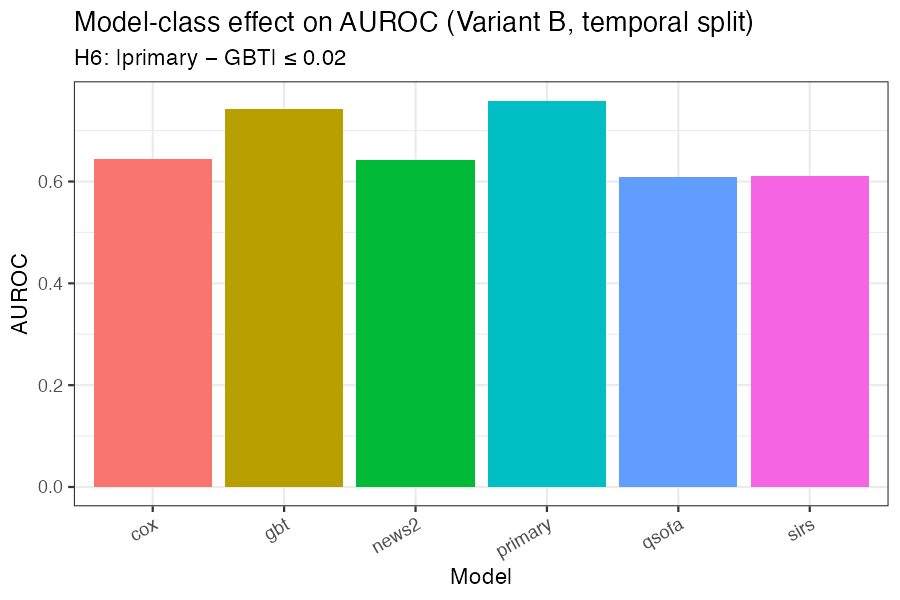
\includegraphics[width=0.85\textwidth]{images/09_model_class_auroc.png}
    \caption{AUROC by model class (Variant B, temporal split). The two flexible
    estimators are close to one another and clearly ahead of the rule-based
    scores and the Cox comparator; on the paired contrast the primary model
    leads GBT by \pcHSixAbsEst{} (Section~\ref{sec:h6}).}
    \label{fig:model_class_auroc}
\end{figure}
